\documentclass{beamer}
\usetheme{metropolis}           % Use metropolis theme
\usefonttheme[onlymath]{serif}
\usepackage{amsmath}
\usepackage{graphicx}
\usepackage{tikz}
\usepackage[style=authortitle,backend=bibtex]{biblatex}

\usetikzlibrary{calc,trees,positioning,arrows,chains,shapes.geometric,%
	decorations.pathreplacing,decorations.pathmorphing,shapes,%
	matrix,shapes.symbols,decorations.markings}
\tikzset{
	>=stealth',
	punktchain/.style={
		rectangle, 
		rounded corners, 
		% fill=black!10,
		draw=black, very thick,
		text width=7em, 
		minimum height=3em, 
		text centered, 
		on chain},
	line/.style={draw, thick, <-},
	element/.style={
		tape,
		top color=white,
		bottom color=blue!50!black!60!,
		minimum width=8em,
		draw=blue!40!black!90, very thick,
		text width=6em, 
		minimum height=3.5em, 
		text centered, 
		on chain},
	every join/.style={->, thick,shorten >=2pt},
	decoration={brace,mirror, amplitude=5pt},
	tuborg/.style={decorate},
	tubnode/.style={midway, right=2pt},
}


\tikzstyle{roundrect}=[rectangle, rounded corners, minimum width=3cm, minimum height=1cm, text centered, draw=black, fill=nodeColor, text width=5cm] 
\tikzstyle{roundrectSmall}=[rectangle, rounded corners, minimum width=0.2cm, minimum height=0.7cm, text centered, draw=black, fill=nodeColor, text width=1.8cm] 
\tikzstyle{roundrectSmallLong}=[rectangle, rounded corners, minimum width=0.2cm, minimum height=0.7cm, text centered, draw=black, fill=nodeColor, text width=3cm] 

\tikzstyle{decision} = [diamond, minimum width=3.7cm, minimum height=3.2cm, text centered, draw=black, fill=decisionColor, scale=1, text width=2.05cm]
\tikzstyle{arrow} = [decoration={markings,mark=at position 1 with
	{\arrow[scale=1.5,>=stealth]{>}}},postaction={decorate}]
%https://tex.stackexchange.com/questions/50780/arrows-at-right-angles-on-a-tikzpicture-matrix
\tikzset{
	desicion/.style={
		diamond,
		draw,
		text width=3em,
		text badly centered,
		inner sep=0pt
	},
	block/.style={
		rectangle,
		draw,
		text width=10em,
		text centered,
		rounded corners
	},
	cloud/.style={
		draw,
		ellipse,
		minimum height=2em
	},
	descr/.style={
		fill=white,
		inner sep=2.5pt
	},
	connector/.style={
		-latex
	},
	rectangle connector/.style={
		connector,
		to path={(\tikztostart) -- ++(#1,0pt) \tikztonodes |- (\tikztotarget) },
		pos=0.5
	},
	rectangle connector/.default=-2cm,
	straight connector/.style={
		connector,
		to path=--(\tikztotarget) \tikztonodes
	}
}

\setbeamertemplate{caption}{\insertcaption}

\usepackage{cancel}
\renewcommand\CancelColor{<color command>}
\usepackage{xcolor}
\newcommand\Ccancel[2][black]{\renewcommand\CancelColor{\color{#1}}\cancel{#2}}

\definecolor{bluenewcolor}{RGB}{20,20,100}
\definecolor{greennewcolor}{RGB}{0,100,0}
\definecolor{decisionColor}{HTML}{DEE1B2}
\definecolor{nodeColor}{HTML}{EBFAFF}
\def\mathunderline#1#2{\color{#1}\underline{{\color{black}#2}}\color{black}}


\title{Master Thesis Presentation\\
STOCHASTIC APPROACH TO MANY-BODY PROBLEMS}
\date{\today}
\author{Anna Gribkovakaya}
\institute{University of Oslo}
\titlegraphic{
	\begin{picture}(0,0)
	\put(300,-125){\makebox(0,0)[rt]{
\includegraphics[width=3cm]{UiOlogo}}}
	\end{picture}}

\begin{document}
  \maketitle
  \section{Introduction}
   \begin{frame}{Outline}
   \begin{itemize}
   	\item Main Objectives
   		\item Many-body problem formulation and Size of the Hilbert Space
   	\item Many body \textit{Ab initio} methods: deterministic and stochastic
   	\item Coupled Cluster Theory
   	\item Coupled Cluster Quantum Monte Carlo
   	\item Results
   	\item Summary
   \end{itemize}
 \end{frame}
   \begin{frame}{Objectives}
	The main objectives:
	\begin{itemize}
 	\item Implement numerical methods to solve the Time Independent Schr\"{o}dinger equation for N electrons
 	\item Develop a Coupled Cluster Doubles code capable of handling relatively large systems
 	\item The code should be general and can be applied to other systems
 	\item Develop a Stochastic Coupled Cluster Doubles code
 	\item Benchmarking with other methods
	\end{itemize}
	\end{frame}


  \section{Main Part}
  
\begin{frame}{Many-body: problem formulation}
The Hamiltonian for quantum mechanical system consisting of N particles  can be written as
\begin{equation*}
\hat{H} = -\frac{1}{2}\sum_{i=1}^{N} \nabla_i^2 + \sum_{i<j}^{N}\frac{1}{r_{ij}} + \sum_{i=1}^{N} \hat{V}_{\text{external}}(r_i),
\end{equation*}
$r_{ij}$  relative distance between the particles, \\
$\hat{V}_{\text{external}}(r_i)$ external one-body potential.\\

Stationary Schr\"{o}dinger equation can be written as:
\begin{equation*}
\hat{H}\Psi_n(\vec{\textbf{R}}) = E_n\Psi_n(\vec{\textbf{R}}),
\end{equation*}
$\vec{\textbf{R}}$ - vector representing both coordinates and spins for all particles.
\begin{equation*}
\vec{\textbf{R}} = \{\vec{R_n}\}= \{(\vec{r}, \sigma)_n\},
\end{equation*}
For fermions the wave function must be antisymmetric:
\begin{equation*}
\Psi_n({\dots, \vec{R}_p , \dots, \vec{R}_q, \dots}) = -\Psi_n({\dots, \vec{R}_q , \dots, \vec{R}_p, \ \dots}),
\end{equation*}
\end{frame}

\begin{frame}{Many-body: Slater Determinant Space}
\begin{itemize}
  	\item Slater Determinant (SD) Space is a Hilbert space for fermions 
  	\item Each SD is constructed from $N$ orthonormal single particle
  	wavefunctions
  	\item SD for reference vacuum state :
  \begin{equation*}
  |D_0\rangle = \frac{1}{\sqrt{N!}}
  \left| \begin{array}{ccccc} \psi_{1}(x_1)& \psi_{1}(x_2)& \dots & \psi_{1}(x_N)\\
  \psi_{2}(x_1)&\psi_{2}(x_2)& \dots  & \psi_{2}(x_N)\\  
  \vdots & \vdots & \ddots  & \vdots \\
  \psi_{N}(x_1)&\psi_{N}(x_2)& \dots  & \psi_{N}(x_N)\end{array} \right| 
  \end{equation*}
  \item Every  SD is anti-symmetric by construction
   \end{itemize}
  \end{frame}

 \begin{frame}{Many-body: Size of the Slater Determinant Space}
An orthonormal set of 2M spin-orbitals, where N are occupied.
\begin{equation*}
\binom {2M}{N} = \frac{(2M)!}{N!(2M-N)!}, 
\end{equation*}
\begin{center}
	\begin{columns}
		\begin{column}{0.5\textwidth}
For the electron gas, $N$=14:   \\
$2M$=38 ($N_s$=3)  	$\rightarrow$ $10^{10}$ \\
$2M$=246 ($N_s$=10)	$\rightarrow$ $10^{22}$\\
$2M$=730 ($N_s$=20)	$\rightarrow$ $10^{29}$
		\end{column}
		\begin{column}{0.5\textwidth}  %%<--- here
			For Quantum Dot, $N$=20:   \\
			$2M$=110 ($N_s$=10)  	$\rightarrow$ $10^{21}$ \\
			$2M$=420 ($N_s$=20)	$\rightarrow$ $10^{33}$\\
			$2M$=930 ($N_s$=30)	$\rightarrow$ $10^{40}$,
		\end{column}
	\end{columns}
\end{center}
here $N_s$ is shell number.
\end{frame}

  \begin{frame}{Many-body: \textit{Ab initio} quantum many body methods}
\uncover<1->{Deterministic Wave Function Methods}
\uncover<1->{ \begin{itemize}
		\item Hartree-Fock Method
		\item Many Body Perturbation Theory
		\item Full Configuration Interaction 
		\item Coupled Cluster Method
\end{itemize}}
\uncover<2->{Stochastic or Monte Carlo (MC) Methods}
\uncover<2->{	\begin{itemize}
		\item Variational MC
		\item Diffusion MC
		\item Full Configuration MC
		\item Coupled Cluster MC
\end{itemize}}
\uncover<3->{Density Functional Theory}
\end{frame}



\section{Coupled Cluster Theory}

  \begin{frame}{Coupled cluster theory: Exponential ansatz}
  The Coupled Cluster approximation for wavefunction is:
	\begin{equation*}
	\Psi_{CC} =  e^{\hat{T}}|D_0\rangle,
	\end{equation*}
	\begin{equation*}
	\hat{T} = \sum_i^{N} \hat{T}_i  = \hat{T}_1 + \hat{T}_2 +\hat{T}_3 + \dots + \hat{T}_N,
	\end{equation*}
	Each excitation operator can be written in terms of creation and annihilation operators:
	\[ 
	\hat{T}_1 = \sum_{i}\hat{t}_i = \sum_{ia}t_{i}^{a} c^\dag_{a}  c_{i}, \text{    } 
	\hat{T}_2 = \sum_{i<j}\hat{t}_{ij}^{ab} = \frac{1}{2!^2}\sum_{ijab}t_{ij}^{ab} c^\dag_{a} c^\dag_{b} c_{j} c_{i}, 
	\]
	\[ 
	\hat{T}_3 = \sum_{i<j<k}\hat{t}_{ijk}^{abc} = \frac{1}{3!^2}\sum_{ijkabc}t_{ijk}^{abc} c^\dag_{a} c^\dag_{b} c^\dag_{c} c_{k}c_{j} c_{i}.
	\,
	\]
	here $i,j,k$ indexes denote the orbitals that are occupied in the reference determinant and $a,b,c$ denote those that are not.
\end{frame}


\begin{frame}
\frametitle{Coupled Cluster: Energy and Amplitudes}
Insert the CC approximation for wave function into TISE:
\begin{equation*}
\hat{H}e^{\hat{T}}|D_0\rangle =Ee^{\hat{T}}|D_0\rangle.
\end{equation*}
\begin{equation*}
\langle D_0|\hat{H}|D_0\rangle +  \langle D_0|\hat{H}\hat{T}|D_0\rangle +\langle D_0|\hat{H}\frac{1}{2!}\hat{T}^2|D_0\rangle  = E.
\end{equation*}
In the energy equation is \textit{naturally truncated} after $\hat{T}^2$.
Equations for the amplitudes can be obtained from:
\begin{equation*}
 \langle D_{ij\dots}^{ab\dots}|\hat{H}e^{\hat{T}}|D_0 \rangle = 0.
\end{equation*}
However for practical purposes we are using so-called similarly transformed Hamiltonian and the equations become:
\begin{equation*}
\text{Energy} \Longrightarrow \langle D_0|e^{-\hat{T}}\hat{H}e^{\hat{T}}|D_0\rangle = E,
\end{equation*}
\begin{equation*}
\text{Amplitudes} \Longrightarrow \langle D_{ij\dots}^{ab\dots}|e^{-\hat{T}}\hat{H}e^{\hat{T}}|D_0 \rangle = 0.
\end{equation*}

\end{frame}


\section{Coupled Cluster Quantum Monte Carlo}

\begin{frame}
\frametitle{Coupled Cluster Quantum Monte Carlo}
CCQMC is a Projector Monte Carlo Method and can be introduced as follows: 
\begin{itemize}
	 \uncover<1->{\item Perform Wick rotation for time dependent Schr\"{o}dinger equation 
	\begin{equation*}
	-i\hbar \frac{\partial}{\partial t} |\Psi(t)\rangle= \hat{H} |\Psi(t)\rangle \Longrightarrow -\frac{\partial}{\partial \tau} |\Psi(\tau)\rangle= \hat{H} |\Psi(\tau)\rangle,
	\end{equation*}}
	\uncover<2->{\item  Express the wave function for arbitrary $\tau$ with a propagator:
	\begin{equation*}
	|\Psi^{(\tau)}\rangle \propto e^{-\tau \hat{H}}|\Psi^{(\tau = 0)}\rangle,
	\end{equation*}}
	\uncover<3->{\item Assume that initial wave function has nonzero overlap with the ground state of the Hamiltonian:
	\begin{equation*}
	|\Psi_0\rangle = \lim_{\tau \rightarrow \infty} e^{-\tau (\hat{H}-S)}|\Psi^{(\tau = 0)}\rangle,
	\end{equation*}}
\end{itemize}
\end{frame}

\begin{frame}{Coupled Cluster Quantum Monte Carlo}

\begin{itemize}
	\uncover<1->{
		\item Approximate the exponential propagator by repeated application of the linear propagator:
		\begin{equation*}
		|\Psi_0\rangle = \lim_{N \rightarrow \infty} \Big[1 - \delta \tau (\hat{H}-S)\Big]^N |\Psi^{(\tau = 0)}\rangle,
		\end{equation*}}
	\uncover<2->{\item  Introduce wave-function for the imaginary time $\tau + \delta \tau$:
		\begin{equation*}
		|\Psi^{(\tau + \delta \tau)}\rangle = (1 - \delta \tau(\hat{H}-S))| \Psi^{(\tau)}\rangle.
		\end{equation*}}
	\uncover<3->{\item Introduce some new notations to simplify equations:
	\[ |D_{\boldsymbol{i}}\rangle = \hat{c}_{\boldsymbol{i}}|D_0\rangle,\]
here $\hat{c}_{\boldsymbol{i}}$ a string of creation and annihilation operators}
\end{itemize}

\end{frame}


\begin{frame}
\frametitle{Coupled Cluster Quantum Monte Carlo}
\begin{itemize}
		\uncover<1->{\item Insert a coupled cluster approximation for the wave function and project equation on the excited determinant $D_{\{\boldsymbol{i}\}}$:}
	\uncover<1->{\begin{align*}
		\langle D_{\{\boldsymbol{i}\}}|e^{\hat{T}}D_0\rangle = \langle D_{\{\boldsymbol{i}\}}|e^{\hat{T}}D_0\rangle - \delta \tau \langle D_{\{\boldsymbol{i}\}}|(\hat{H}-S)e^{\hat{T}}|D_0\rangle,
		\end{align*}}
\uncover<2->{\item Express the RHS of the above equation in terms of amplitudes:}
\uncover<2->{\begin{equation*}
	\langle D_{\boldsymbol{i}}|e^{\hat{T}^{(\tau)}}D_0\rangle = t_{\boldsymbol{i}}^{(\tau)} + \mathcal{O}(\hat{T}^2),
	\end{equation*}}
\uncover<3->{\item Derive the equation for the amplitudes for $\tau+\delta\tau$: 
	\begin{equation*}
	t_{\{\boldsymbol{i}\}}^{(\tau+\delta\tau)}  \only<3>{+\mathcal{O}(\hat{T}^2)\phantom{2}}\only<4>{+\Ccancel[red]{\mathcal{O}(\hat{T}^2)}\phantom{2}}\only<5>{} = t_{\{\boldsymbol{i}\}}^{(\tau)}  \only<3>{+\mathcal{O}(\hat{T}^2)\phantom{2}}\only<4>{+\Ccancel[red]{\mathcal{O}(\hat{T}^2)}\phantom{2}}\only<5>{} - \delta \tau \langle D_{\{\boldsymbol{i}\}}|(\hat{H}-S)e^{\hat{T}}|D_0\rangle,
	\end{equation*}}
\uncover<5->{\item Rewrite it to obtain CCQMC population dynamics equation:
	\begin{equation*}
	\frac{\delta t_{\{\boldsymbol{i}\}}}{\delta\tau} = -\langle D_{\{\boldsymbol{i}\}}|(\hat{H}-S)e^{\hat{T}}|D_0\rangle,
	\end{equation*}}
	\uncover<6->{This looks very similar to the diffusion equation!}	
\end{itemize}
\end{frame}

\begin{frame}
\frametitle{Coupled Cluster Quantum Monte Carlo}
The equation we obtained is very similar to a diffusion one. Now we need to introduce particles or walkers to simulate the population dynamics. We use random walkers to obtain amplitudes. In this case walkers are called ${\color{red}excips}$. 
\begin{equation*}	
\frac{\delta t_{\{\boldsymbol{i}\}}}{\delta\tau} = -\langle D_{\{\boldsymbol{i}\}}|(\hat{H}-S)e^{\hat{T}}|D_0\rangle,
\end{equation*}
Each amplitude corresponds to an excited determinant or ${\color{red}excitor}$. The population of excips on a given excitor is proportional to the amplitude:
\begin{equation*}	
t_{\boldsymbol{i}} \propto N_{\boldsymbol{i}} = \sum_\alpha s_\alpha \delta_{{\boldsymbol{i}}, {\boldsymbol{i}}_\alpha} \text{ and }  N_{ex} = \sum_{\boldsymbol{i}} |N_{\boldsymbol{i}}|
\end{equation*}
here $s_\alpha = \pm 1$ is sign of excip, $t_{\boldsymbol{i}}$ is an amplitude corresponding to the determinant ${{\boldsymbol{i}}_\alpha}$. %The wave function is this case is written as:
%\only<1>{\begin{equation*}
%\Psi_{cc} = \big[1 + \sum_{\boldsymbol{i}} %t_{\boldsymbol{i}}\hat{a}_{\boldsymbol{i}} + \frac{1}{ %2!}\sum_{\boldsymbol{ij}} t_{\boldsymbol{i}} t_{\boldsymbol{j}} %\hat{a}_{\boldsymbol{i}} \hat{a}_{\boldsymbol{j}} + \frac{1}{ %3!}\sum_{\boldsymbol{ijk}}t_{\boldsymbol{i}} t_{\boldsymbol{j}} %t_{\boldsymbol{k}} \hat{a}_{\boldsymbol{i}} \hat{b}_{\boldsymbol{j}} %\hat{a}_{\boldsymbol{k}} + ...  \big]|D_0\rangle.
%\end{equation*}}
\end{frame}

\begin{frame}
\frametitle{CCQMC: Game of Life}
CCQMC simulated equation:
\begin{equation*}	
\frac{\delta t_{\{\boldsymbol{i}\}}}{\delta\tau} = -\langle D_{\{\boldsymbol{i}\}}|(\hat{H}-S)e^{\hat{T}}|D_0\rangle,
\end{equation*}
Exponential ansatz:
\begin{equation*}
\Psi_{cc} = \big[1 + \sum_{\boldsymbol{i}} t_{\boldsymbol{i}}\hat{a}_{\boldsymbol{i}} + \frac{1}{ 2!}\sum_{\boldsymbol{ij}} t_{\boldsymbol{i}} t_{\boldsymbol{j}} \hat{a}_{\boldsymbol{i}} \hat{a}_{\boldsymbol{j}} + \frac{1}{ 3!}\sum_{\boldsymbol{ijk}}t_{\boldsymbol{i}} t_{\boldsymbol{j}} t_{\boldsymbol{k}} \hat{a}_{\boldsymbol{i}} \hat{a}_{\boldsymbol{j}} \hat{a}_{\boldsymbol{k}} + ...  \big]|D_0\rangle.
\end{equation*}
After the wave function collapse:
\begin{equation*}	
\frac{\delta t_{\{\boldsymbol{i}\}}}{\delta\tau} = -\langle D_n|(\hat{H}-S)|D_m\rangle,
\end{equation*}
These determinants are connected through the Hamiltonian.
\end{frame}


\begin{frame}
\frametitle{CCQMC: Game of Life}
Probability to spawn:
\begin{equation*}
P_{\text{spawn}} =\delta \tau |A H_{nm}| \frac{1}N_a p_{size}(s) p_{clust} (e|s)\frac{1}{p_{gen}},
\end{equation*}
Probability do die:
\begin{equation*}
P_{\text{death}} = \delta \tau | A (H_{mm}-S) | \frac{1}{N_a p_{size}(s) p_{clust} (e|s)} .
\end{equation*}
\end{frame}

\begin{frame}
\frametitle{CCQMC: Game of Life}
Probabilities:
\begin{align*}
&p_{size}(s)=\frac{1}{2^{s+1}},\\
&A = N_0 \sum_{i=1}^{s} \frac{N_i}{N_0}, \\
&p_{clust} (e|s)=s! \prod_{i=1}^{s}\frac{|N_i|}{N_{ex}},\\
&p_{gen}=p(r,s|p,q)p(p,q), \ \ \ p(p,q) = \binom{N}{2}^{-1}\\
&p(r,s|p,q)=p(r|s, p,q)p(s|p,q) + p(s|r, p,q)p(r|p,q).
\end{align*}
\end{frame}


\begin{frame}
\frametitle{First Iteration}
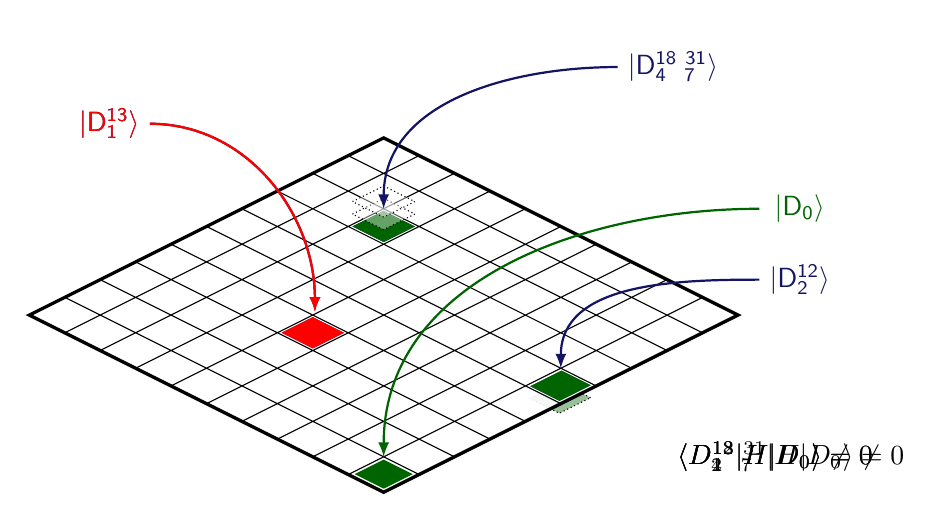
\begin{tikzpicture}[scale=.9,every node/.style={minimum size=1cm},on grid]
\begin{scope}[
yshift=-5,every node/.append style={
	yslant=0.5,xslant=-1},yslant=0.5,xslant=-1
]
\uncover<10->{\fill[greennewcolor,fill opacity=.4] (2.97,0.05) rectangle (2.53,0.46);}
\uncover<10->{\draw[black,densely dotted] (2.97,0.05) rectangle (2.53,0.46);}
\end{scope}

\begin{scope}[
yshift=0,every node/.append style={
	yslant=0.5,xslant=-1},yslant=0.5,xslant=-1
]
\fill[white,fill opacity=.9] (0,0) rectangle (5,5);
\draw[black,very thick] (0,0) rectangle (5,5);
\draw[step=5mm, black] (0,0) grid (5,5);
\uncover<2->{\fill[greennewcolor] (0.05,0.05) rectangle (0.46,0.46);}
\uncover<3>{\fill[bluenewcolor] (1.97,2.97) rectangle (1.53,2.53);}
\uncover<4>{\fill[red] (1.97,2.97) rectangle (1.53,2.53);}
\uncover<5>{\fill[bluenewcolor] (3.97,3.97) rectangle (3.53,3.53);}
\uncover<6->{\fill[greennewcolor] (3.97,3.97) rectangle (3.53,3.53);}
\uncover<9>{\fill[bluenewcolor] (2.97,0.05) rectangle (2.53,0.46);}
\uncover<10->{\fill[greennewcolor] (2.97,0.05) rectangle (2.53,0.46);}
\end{scope}

\begin{scope}[
yshift=5,every node/.append style={
	yslant=0.5,xslant=-1},yslant=0.5,xslant=-1
]
\uncover<7->{\fill[white,fill opacity=.4] (3.97,3.97) rectangle (3.53,3.53);}

\uncover<7->{\draw[black,densely dotted] (3.97,3.97) rectangle (3.53,3.53);}
\end{scope}

\begin{scope}[
yshift=10,every node/.append style={
	yslant=0.5,xslant=-1},yslant=0.5,xslant=-1
]
\uncover<8->{\fill[white,fill opacity=.4] (3.97,3.97) rectangle (3.53,3.53);}

\uncover<8->{\draw[black,densely dotted] (3.97,3.97) rectangle (3.53,3.53);}
\end{scope}
\uncover<2->{\draw[-latex,thick,greennewcolor](5.3,4.0)node[right]{$\mathsf{|D_0\rangle}$}
	to[out=180,in=90] (0,0.5);}
\uncover<3>{\draw[-latex,thick,bluenewcolor](-3.3,5.2)node[left]{$\mathsf{|D_{1}^{13}\rangle}$}
	to[out=0,in=90] (-0.97,2.55);}
\uncover<4>{\draw[-latex,thick,red](-3.3,5.2)node[left]{$\mathsf{|D_{1}^{13}\rangle}$}
	to[out=0,in=90] (-0.97,2.55);}

\uncover<5->{\draw[-latex,thick,bluenewcolor](3.3,6.0)node[right]{$\mathsf{|D_{4\ \ 7}^{18 \ 31}\rangle}$}
	to[out=180,in=90] (0,4.0);}
\uncover<9->{\draw[-latex,thick,bluenewcolor](5.3,3.0)node[right]{$\mathsf{|D_2^{12}\rangle}$}
	to[out=180,in=90] (2.5,1.75);}

\uncover<4>{\draw[thick,black](4.0,0.5)node[right]{$\langle D_1^{13}|H|D_0\rangle = 0$};}
\uncover<5>{\draw[thick,black](4.0,0.5)node[right]{$\langle D_{4\ \ 7}^{18 \ 31}|H|D_0\rangle \neq 0$};}
\uncover<10>{\draw[thick,black](4.0,0.5)node[right]{$\langle D_2^{12}|H|D_0\rangle \neq 0$};}
\end{tikzpicture}
\begin{equation*}
\only<1-6>{\Big[ D_0 \mid  \dots \Big]}\phantom{7}\only<7-9>{\Big[ D_0 \mid D_{4\ \ 7}^{18 \ 31} \mid \dots \Big]}\only<10->{\Big[ D_0 \mid D_{4\ \ 7}^{18 \ 31} \mid D_2^{12} \mid \dots \Big]}
\end{equation*}
\begin{equation*}
\only<1-6>{\Big[N_0 \mid \dots \Big]}\phantom{7}\only<7>{\Big[N_0 \mid \ \ +1 \ \ \mid \dots \Big]}\only<8-9>{\Big[N_0 \mid \ \ +2 \ \ \mid \dots \Big]}\only<10->{\Big[N_0 \mid \ \ +2 \ \ \mid  -1 \ \ \mid \dots \Big]}
\end{equation*}
\end{frame}


\begin{frame}
\frametitle{Iteration}
		
			\begin{align*}	
			\only<1,9,17>{-\langle D_{\{\boldsymbol{i}\}}|(\hat{H}-S)|\Psi_{cc}\rangle}\vphantom{\langle \underline{D_{\{\boldsymbol{i}\}}}|(\hat{H}-S)|D_n\rangle}
			\only<2-3,10,18-21>{-\langle D_{\{\boldsymbol{i}\}}|(\hat{H}-S)|\underline{\Psi_{cc}}\rangle}
			\only<4-5>{-\langle D_{\{\boldsymbol{i}\}}|(\hat{H}-S)|D_n\rangle}
			\only<6>{-\langle \underline{D_{\{\boldsymbol{i}\}}}|(\hat{H}-S)|D_n\rangle}
			\only<7-8>{-\langle D_{m}|(\hat{H}-S)|D_n\rangle}
			\only<11>{-\langle D_{\{\boldsymbol{i}\}}|(\hat{H}-S)|D_{n^\prime}\rangle}
			\only<12>{-\langle \underline{D_{\{\boldsymbol{i}\}}}|(\hat{H}-S)|D_{n^\prime}\rangle}
			\only<13-14>{-\langle D_{m^\prime}|(\hat{H}-S)|D_{n^\prime}\rangle}
			\only<15-16>{-\langle D_{m^{\prime\prime}}|(\hat{H}-S)|D_{n^\prime}\rangle}
			\only<22->{-\langle D_i^c |\hat{H}|D_{ijk}^{abc}\rangle}
			\end{align*}
		
			\begin{center}
			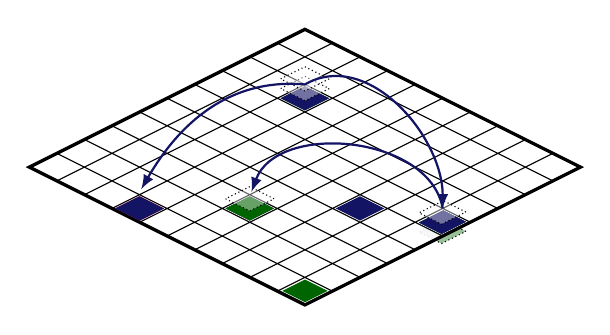
\begin{tikzpicture}[scale=.7,every node/.style={minimum size=1cm},on grid]
			
			%UNDER
			\begin{scope}[
			yshift=-5,every node/.append style={yslant=0.5,xslant=-1},yslant=0.5,xslant=-1]
			\uncover<1-16>{\fill[greennewcolor,fill opacity=.4] (2.97,0.05) rectangle (2.53,0.46);}
			\uncover<1-16>{\draw[black,densely dotted] (2.97,0.05) rectangle (2.53,0.46);}
			\end{scope}
			
			%MAIN
			\begin{scope}[yshift=0,every node/.append style={yslant=0.5,xslant=-1},yslant=0.5,xslant=-1]
			\fill[white,fill opacity=.9] (0,0) rectangle (5,5);
			\draw[black,very thick] (0,0) rectangle (5,5);
			\draw[step=5mm, black] (0,0) grid (5,5);
			\uncover<1->{\fill[greennewcolor] (0.05,0.05) rectangle (0.46,0.46);}
			\uncover<1->{\fill[greennewcolor] (3.97,3.97) rectangle (3.53,3.53);}
			\uncover<11-15>{\fill[bluenewcolor] (3.97,3.97) rectangle (3.53,3.53);}
			\uncover<1-16>{\fill[greennewcolor] (2.97,0.05) rectangle (2.53,0.46);}
			\uncover<4-8>{\fill[bluenewcolor] (2.97,0.05) rectangle (2.53,0.46);}
			\uncover<7>{\fill[bluenewcolor] (1.47,2.03) rectangle (1.03,2.47);}
			\uncover<8->{\fill[greennewcolor] (1.47,2.03) rectangle (1.03,2.47);}
			\uncover<13>{\fill[bluenewcolor] (0.47,3.03) rectangle (0.03,3.47);}
			\uncover<14>{\fill[red] (0.47,3.03) rectangle (0.03,3.47);}
			\uncover<15>{\fill[bluenewcolor] (2.97,0.05) rectangle (2.53,0.46);}
			%composite ket
			\uncover<19->{\fill[bluenewcolor] (0.47,3.03) rectangle (0.03,3.47);}
			%composite bra
			\uncover<21->{\fill[bluenewcolor] (2.47,1.03) rectangle (2.03,1.47);}
			\end{scope}
			%ABOVE		
			\begin{scope}[
			yshift=5,every node/.append style={yslant=0.5,xslant=-1},yslant=0.5,xslant=-1]
			\uncover<1->{\fill[white,fill opacity=.4] (3.97,3.97) rectangle (3.53,3.53);}
			\uncover<1->{\draw[black,densely dotted] (3.97,3.97) rectangle (3.53,3.53);}
			\uncover<8->{\fill[white,fill opacity=.4] (1.47,2.03) rectangle (1.03,2.47);}
			\uncover<8->{\draw[black,densely dotted] (1.47,2.03) rectangle (1.03,2.47);}
			\uncover<16>{\fill[white,fill opacity=.4] (2.97,0.05) rectangle (2.53,0.46);}
			\uncover<16>{\draw[black,densely dotted] (2.97,0.05) rectangle (2.53,0.46);}
			\end{scope}
			%ABOVE#2
			\begin{scope}[
			yshift=10,every node/.append style={yslant=0.5,xslant=-1},yslant=0.5,xslant=-1]
			\uncover<1-16>{\fill[white,fill opacity=.4] (3.97,3.97) rectangle (3.53,3.53);}
			\uncover<1-16>{\draw[black,densely dotted] (3.97,3.97) rectangle (3.53,3.53);}
			\end{scope}
			
			
			%HAMILTONIAN
			\uncover<7-8>{\draw[-latex,thick,bluenewcolor](2.5,1.75)node[right]{}to[out=100,in=70] (-0.97,2.05);}
			\uncover<13-14>{\draw[-latex,thick,bluenewcolor](0,4.0)node[right]{} to[out=175,in=60] (-2.97,2.10);}
			\uncover<15> {\draw[-latex,thick,bluenewcolor](0,4.0)node[right]{} to[out=30,in=90] (2.5,1.75);}
			
			\end{tikzpicture}
		\end{center}	
\begin{equation*}
\Psi_{cc} = \big[1 +\only<1-2,18->{\sum_{\boldsymbol{i}} t_{\boldsymbol{i}}\hat{a}_{\boldsymbol{i}}\vphantom{\underbrace{\sum_{\boldsymbol{i}} t_{\boldsymbol{i}}\hat{a}_{\boldsymbol{i}}}_\text{size one}}}\only<3-17>{\underbrace{\sum_{\boldsymbol{i}} t_{\boldsymbol{i}}\hat{a}_{\boldsymbol{i}}}_\text{size one}}+
\only<1-17>{\sum_{\boldsymbol{ij}} t_{\boldsymbol{i}} t_{\boldsymbol{j}} \hat{a}_{\boldsymbol{i}} \hat{a}_{\boldsymbol{j}}}\vphantom{\underbrace{\sum_{\boldsymbol{ij}} t_{\boldsymbol{i}} t_{\boldsymbol{j}} \hat{a}_{\boldsymbol{i}} \hat{a}_{\boldsymbol{j}}}_\text{size two}}
\only<18->{\underbrace{\sum_{\boldsymbol{ij}} t_{\boldsymbol{i}} t_{\boldsymbol{j}} \hat{a}_{\boldsymbol{i}} \hat{a}_{\boldsymbol{j}}}_\text{size two}}
+ \sum_{\boldsymbol{ijk}}t_{\boldsymbol{i}} t_{\boldsymbol{j}} t_{\boldsymbol{k}} \hat{a}_{\boldsymbol{i}} \hat{a}_{\boldsymbol{j}} \hat{a}_{\boldsymbol{k}} + ...  \big]|D_0\rangle.
\end{equation*}
\begin{equation*}
\only<18>{\hat{c}_{ik}^{ac} \ -\hat{c}_j^b}
\only<19>{\hat{c}_{ik}^{ac} \ -\hat{c}_j^b \rightarrow -\hat{c}_{ijk}^{abc}}
\only<20>{-\hat{c}_{ijk}^{abc}|D_0\rangle = -|D_{ijk}^{abc}\rangle}
\only<21>{-|D_{ijk}^{abc}\rangle \rightarrow \ \ ^c_i}
\only<22>{\delta\tau \langle D_i^c |\hat{H}|D_{ijk}^{abc}\rangle }
\only<23>{\delta\tau \langle D_{ijk}^{abc} |\hat{H}-S|D_{ijk}^{abc}\rangle }
\end{equation*}
\end{frame}



\section{Results}
\begin{frame}
\frametitle{Benchmarking}
\begin{table}[h]
	\centering
	%\captionsetup{width=.8\textwidth}
	\caption{\tiny CCD(deterministic) results for $14$ electrons. Mixing parameter $\alpha=0.8$ for Miller's results, and $\alpha=0.3$ for our results. All energies are presented in Hartree units.} \label{tab:CCDcompar}
	\tiny  %%  command to change the font size
	\begin{tabular}{rrll}
		$r_s$ & States & $\Delta E_{CCD}$ \footnote{\tiny Quantum Mechanical Studies of Infinite Matter by the Use of Coupled-Cluster Calculations, with an Emphasis on Nuclear Matter. Sean Bruce Sangolt Miller. 2017}  & $\Delta E_{CCD}$\\
		\hline
		\hline
		1.0 & 54 & -0.3178228436889338 & -0.3178230699319593  \\
		1.0 & 66 & -0.3926965898061968 & -0.3926968074770886  \\
		1.0 & 114 & -0.4479105961757175 & -0.4479109389185165  \\
		1.0 & 162 & -0.4805572589306421 & -0.4805570782443642  \\
		1.0 & 186 & -0.4855229317521320 & -0.4855227418241649  \\
		1.0 & 246 & -0.4929245740023971 & -0.4929243692209991  \\
		1.0 & 294 & -0.4984909094066806 & -0.4984906939593084  \\
		1.0 & 342 & -0.5019526761547777 & -0.5019524529049425  \\
		1.0 & 358 & -0.5025196736076414 & -0.5025194488388953  \\ \hline
		0.5 & 114 & -0.5120153541478306 & -0.5120152296730573  \\
		0.5 & 342 & -0.5729645498903680 & -0.572964399507112   \\ \hline    
		2.0 & 114 & -0.3577968843144996 & -0.3577955282575226  \\
		2.0 & 342 & -0.4014136184665558 & -0.4014117905655014  \\
	\end{tabular}
\end{table}
%\begin{thebibliography} 
%	\bibitem[Quantum Mechanical Studies of Infinite Matter by the Use of Coupled-Cluster Calculations, with an Emphasis on Nuclear Matter]{abc}
%\end{thebibliography}

\end{frame}

%\begin{frame}
%\frametitle{Benchmarking}
%\begin{figure}[ht!]
%	\centering
%	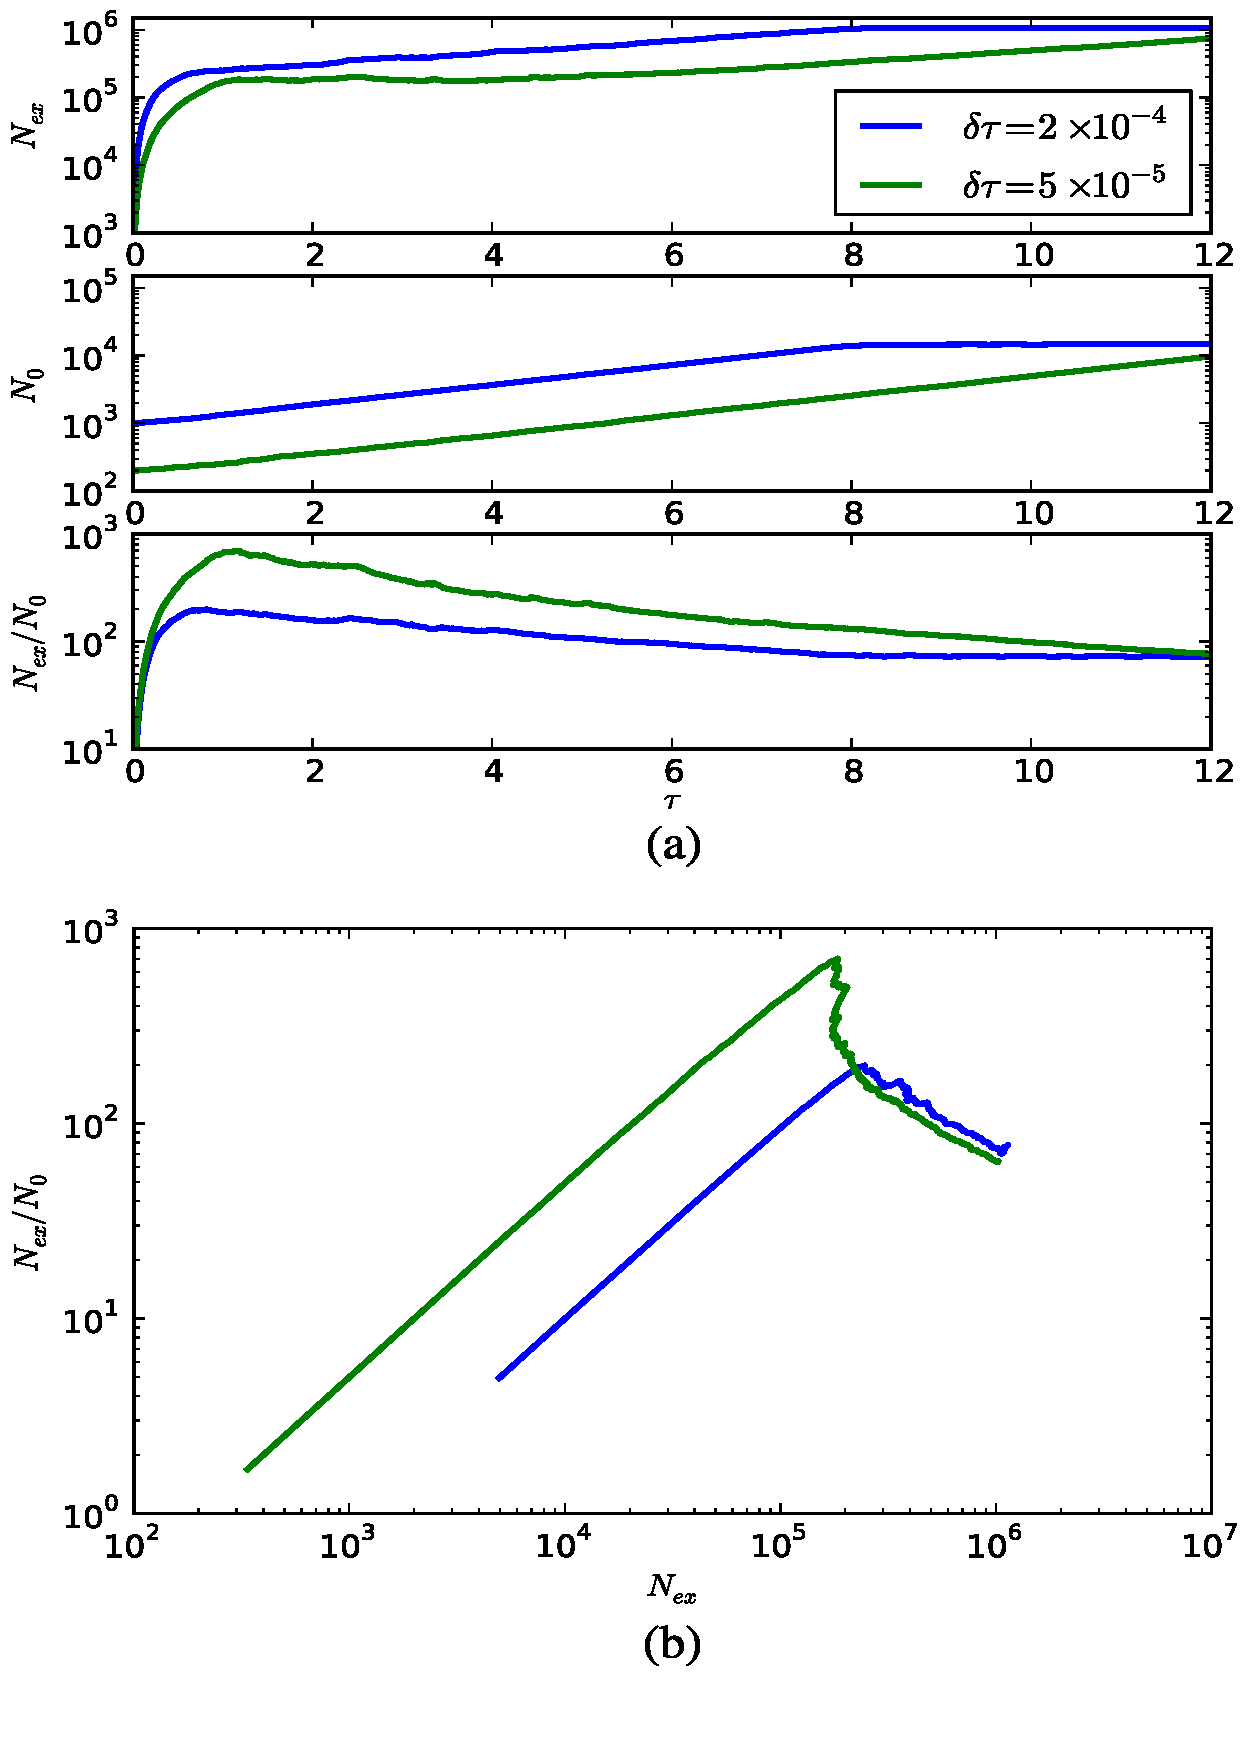
\includegraphics[scale=0.30]{thomEG}
%	\caption{ }
%	%\label{}
%\end{figure}
%\end{frame}
\begin{frame}
\frametitle{Population dynamics}

\begin{columns}
\begin{column}{0.60\textwidth}
	\begin{center}
		\begin{figure}
			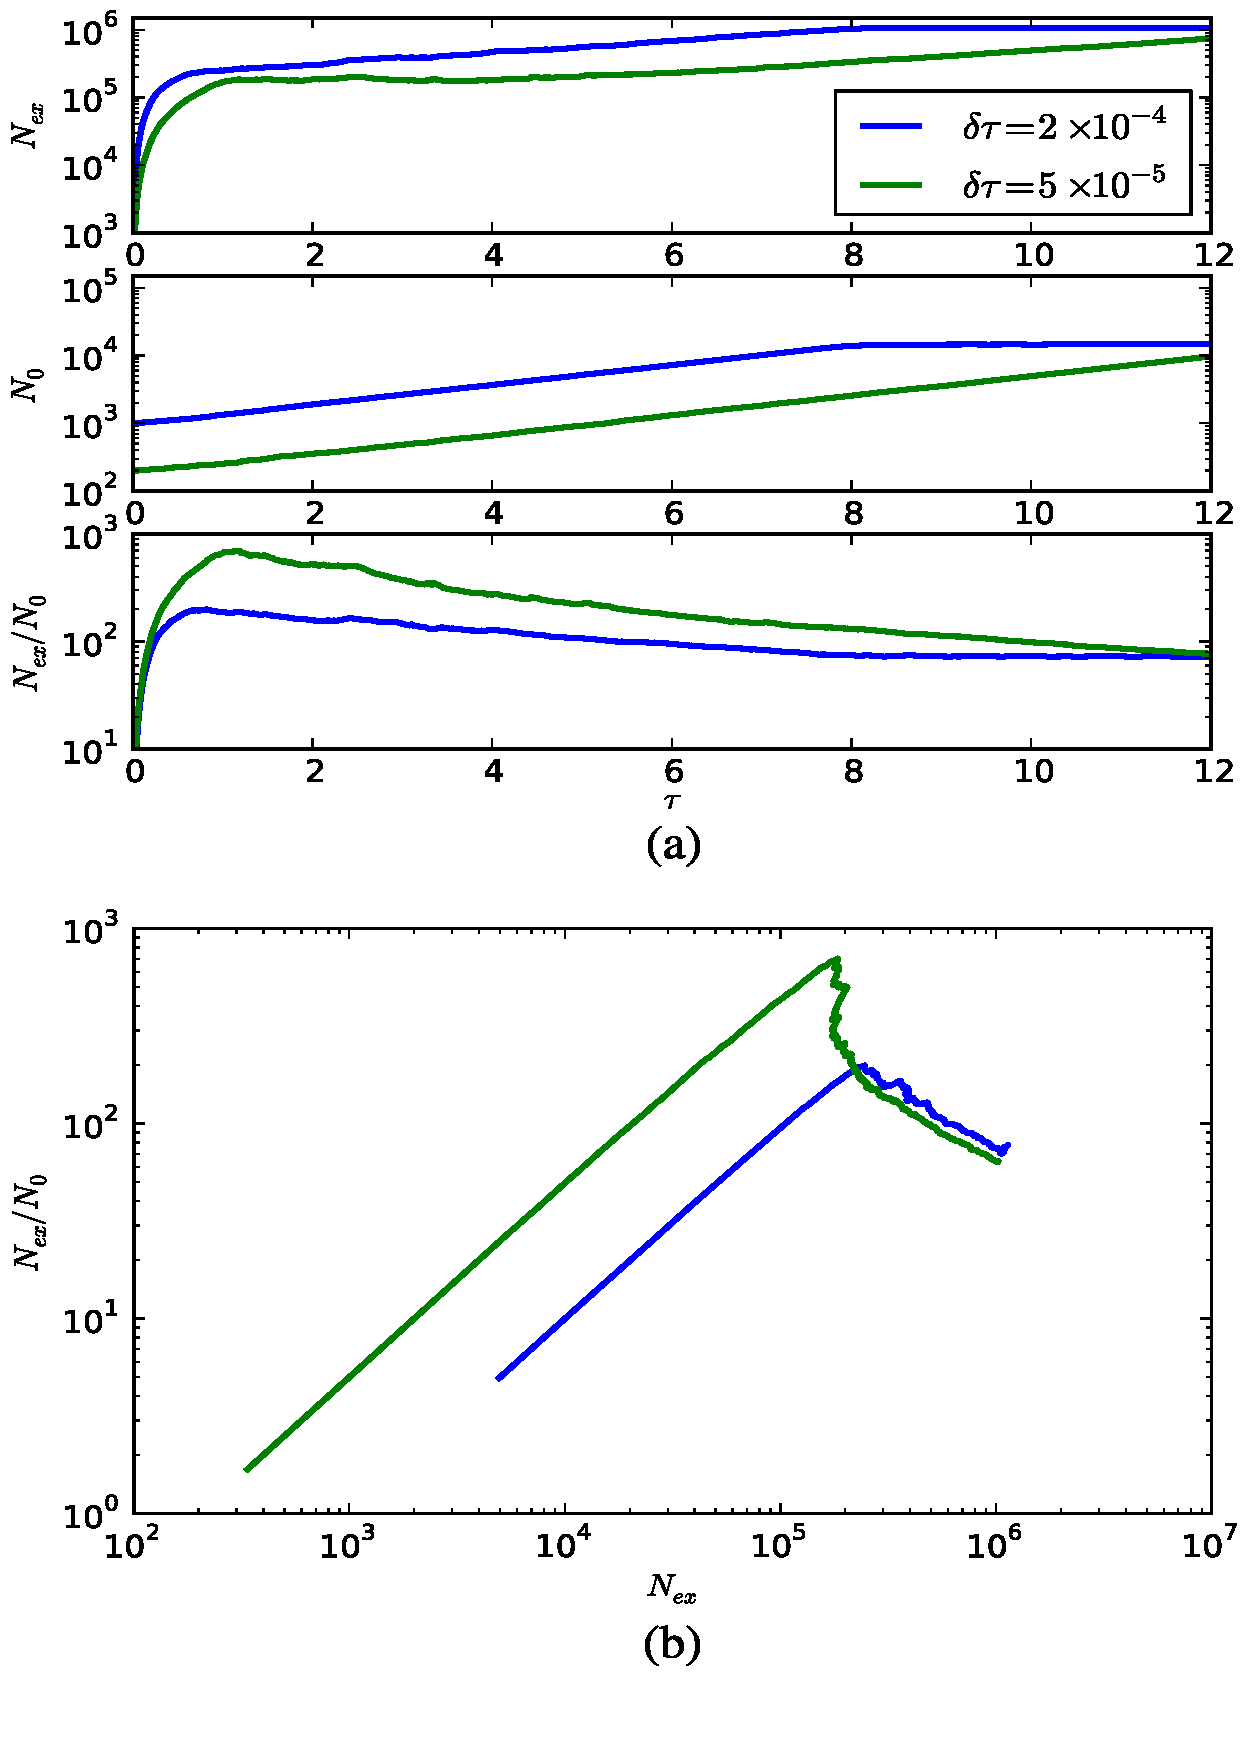
\includegraphics[scale=0.20]{thomEG}
		\end{figure}
	\end{center}
\end{column}
\begin{column}{0.40\textwidth}
	\tiny Ne CCSDTQ calculations starting with different initial
	particle numbers at the reference and different timesteps. (a): With a carefully
	chosen low timestep and initial population, a plateau is visible. An increased
	timestep and initial population overshoot the plateau but have a shoulder.
	The lower panel shows a maximum of the particle ratio at the position of the
	shoulder and plateau. (b): "Shoulder plots" allow shoulder height to be read off
	easily.  \footnote{\tiny James S. Spencer and Alex J. W. Thom. “Developments in\\ Stochastic
		Coupled Cluster Theory: The Initiator Approximation\\ and Application to the
		Uniform Electron Gas”.\\ The Journal of Chemical Physics 144.8 (Feb.
		2016)}
\end{column}
\end{columns}	
\end{frame}

\begin{frame}
\frametitle{Population dynamics}

\begin{columns}
\begin{column}{0.48\textwidth}
\begin{center}
	\begin{figure}
		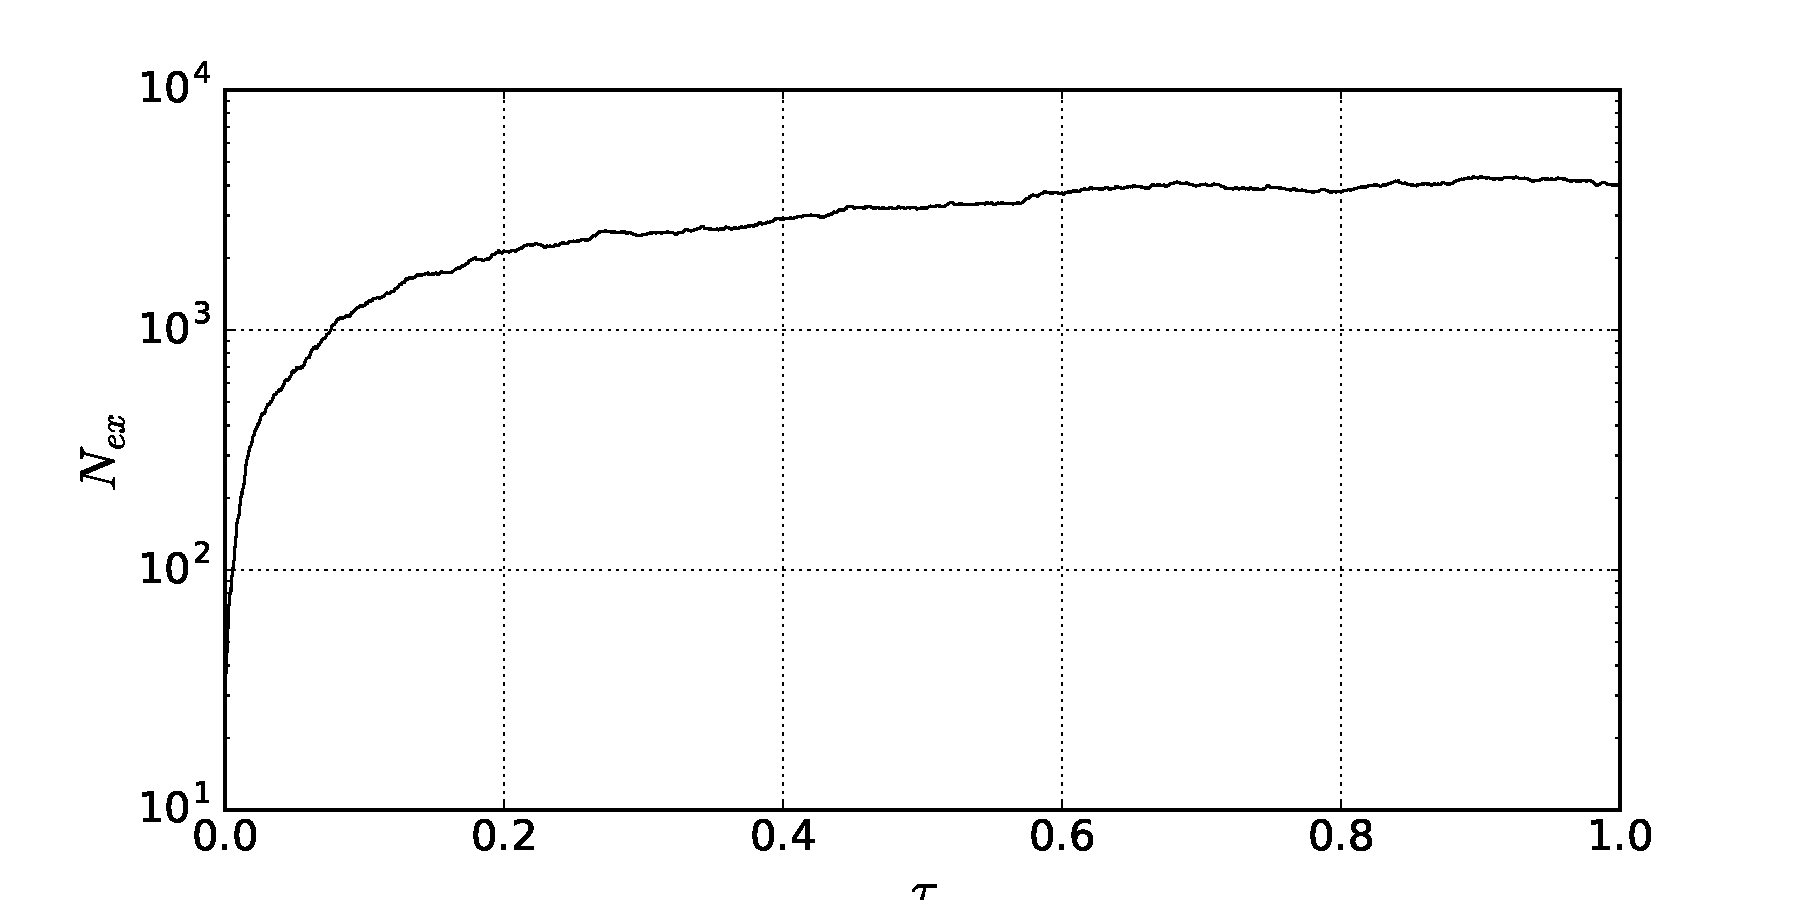
\includegraphics[scale=0.20]{Nex2000new}
	\end{figure}
\end{center}
\end{column}
\begin{column}{0.48\textwidth}
\begin{center}
	\begin{figure}
		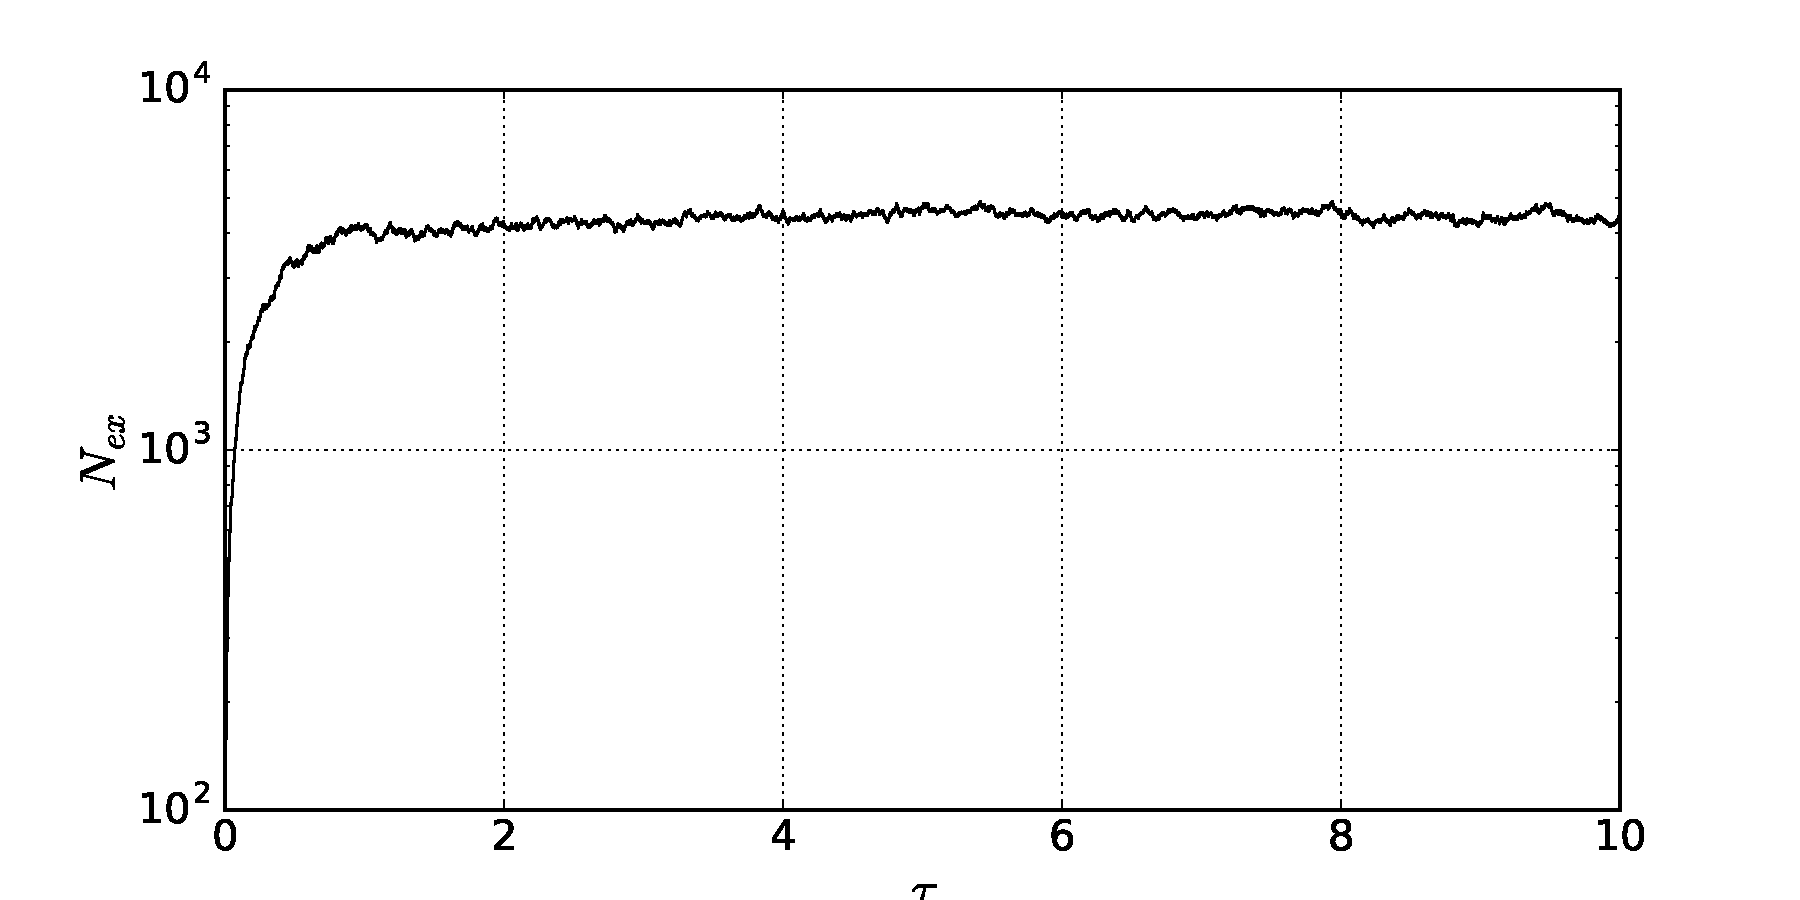
\includegraphics[scale=0.20]{Nex20000}
	\end{figure}
\end{center}
\end{column}
\end{columns}
\tiny The population dynamics of the excited space for 14 electrons and 54 basis functions. $r_s=0.5$, $\delta \tau=0.0005$(left).
The population dynamics of the excited space for 14 electrons and 54 basis functions with $r_s=0.5$, $\delta \tau=0.0005$ and the population control enabled after $5\cdot 10^3$ iterations. Dampening parameter is $\gamma = 0.05$. The energy shift $S$ is tuned every five iterations.(right) 	
\end{frame}

\begin{frame}
\frametitle{Population dynamics}
\begin{figure}[ht!]		
\centering
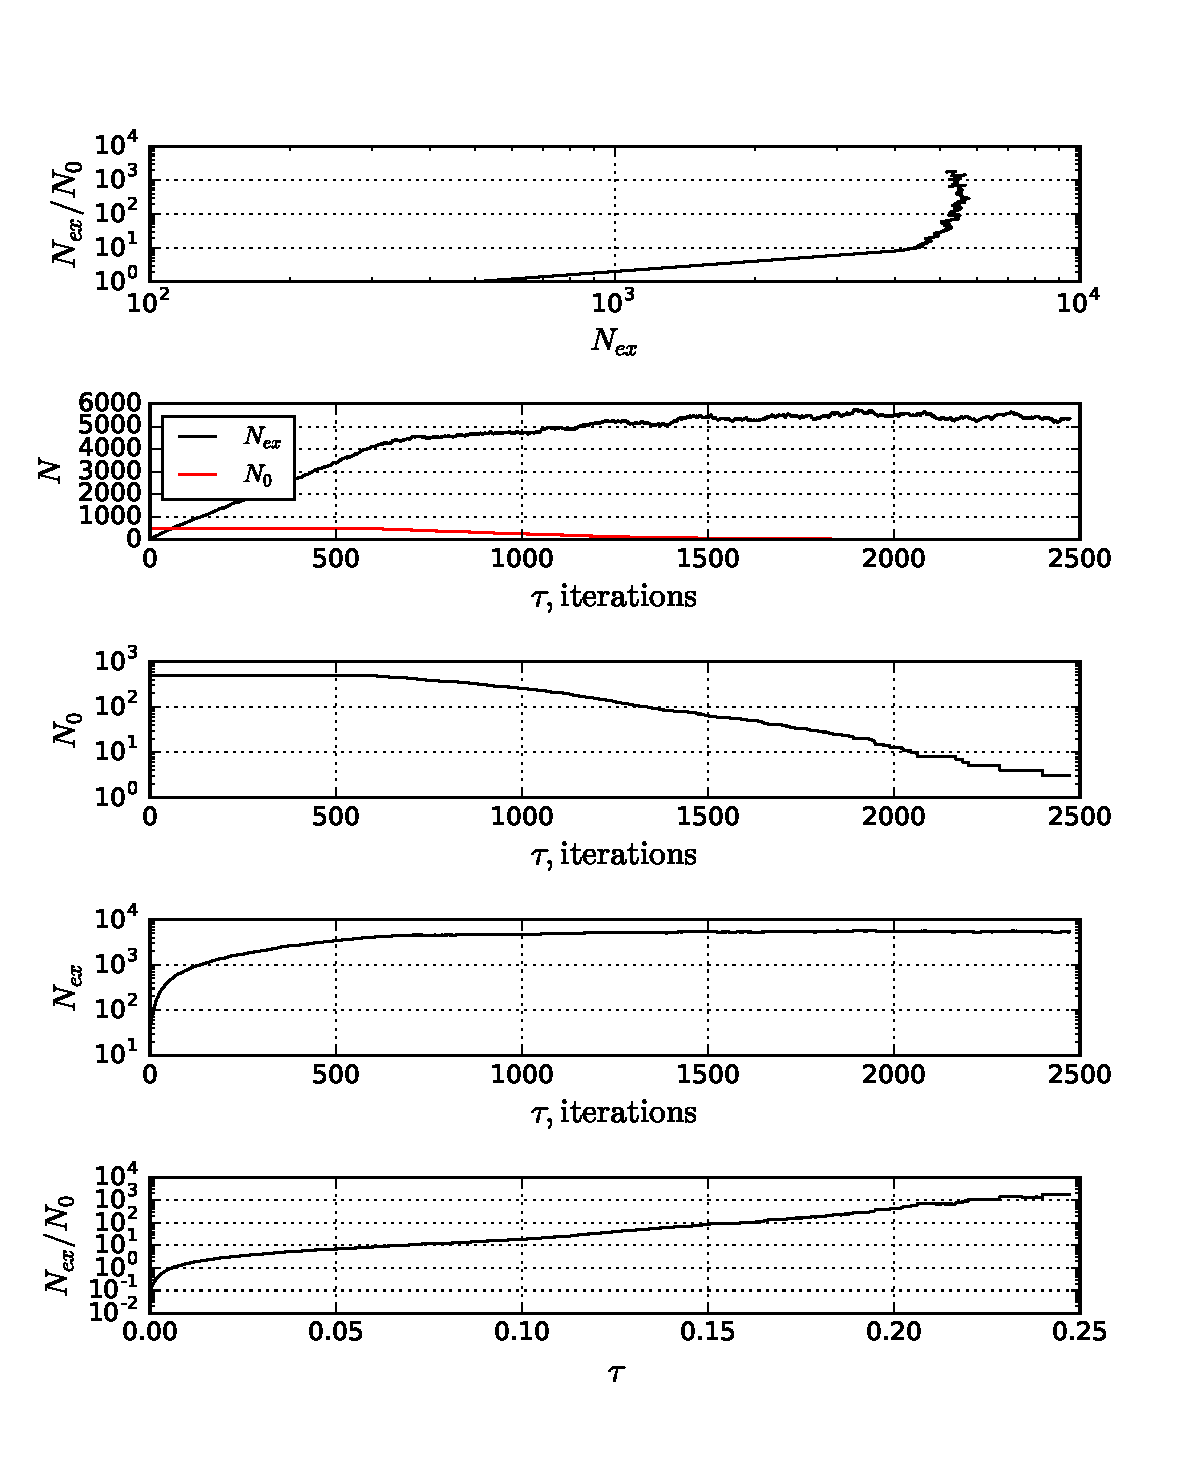
\includegraphics[scale=0.30]{deathN0}
\caption{ }
\label{fig:thomEG}
\end{figure}
\end{frame}


\begin{frame}
\frametitle{CBS energies}
\begin{table}[h]
\centering
\caption{\tiny Summary of complete basis set extrapolated results for the correlation energy of the 14 electron uniform electron gas in hartree. $r_s = 1.0$} \label{tab:CCDQMC}
\tiny  %%  command to change the font size
\begin{tabular}{ll}
$-$ &  $\Delta E_{CCD}$ \\
\hline
\hline
dCCD & -0.514204 \\
dCCD\footnote{\tiny J. J. Shepherd, A. Grüneis, G. H. Booth, G. Kresse, and A. Alavi, Phys. Rev. B 86, 035111 (2012)} & -0.5152(5) \\
\hline
qCCSD\footnote{\tiny Verena A. Neufeld and Alex J. W. Thom. "A Study of the Dense Uniform Electron Gas with High Orders of Coupled Cluster". The Journal of Chemical Physics 147.19 (Nov. 2017)} & -0.51450(9) \\
qCCSDT$^3$ & -0.5307(2) \\
qCCSDTQ$^3$ & -0.5307(2) \\			
\hline
FCIQMC\footnote{\tiny J. J. Shepherd, G. H. Booth, and A. Alavi, J. Chem. Phys. 136, 244101 (2012)} & -0.5325(4) \\
\hline     
\end{tabular}
\end{table}
%\begin{thebibliography} 
%	\bibitem[Quantum Mechanical Studies of Infinite Matter by the Use of Coupled-Cluster Calculations, with an Emphasis on Nuclear Matter]{abc}
%\end{thebibliography}

%\footnote{\tiny Verena A. Neufeld and Alex J. W. Thom. "A Study of the Dense Uniform Electron Gas with High Orders of Coupled Cluster". The Journal of Chemical Physics 147.19 (Nov. 2017)}
\end{frame}


\section{Conclusion}

\begin{frame}
\frametitle{Conclusion}
\begin{itemize}
\item We have developed a CCD solver that reproduced published results for the homogeneous electron gas.
\item This solver can also be applied to other systems.
\item We have used this implementation to obtain a significant benchmark information to develop the CCQMC solver.
\item We have developed a CCQMC solver and found that population of the reference state and truncation level play major roles for the CCQMC algorithm.
\item The CCQMC method allows us to overcome the rapid growth of space size associated with deterministic methods.
\end{itemize}
\end{frame}

\section{Future work}
\begin{frame}
\frametitle{Future work}
\begin{itemize}
\item Implement the method for a higher truncation level.
\item Investigate different sampling schemes.
\item Use optimization techniques, for example initiator approximation.
\item Optimize the implementation both numerically and algorithmically.
\item Use solver for systems.
\end{itemize}
\end{frame}


\section{Back Up Slide}
\begin{frame}
\frametitle{Sing}
Possible sing change can occur:
\begin{itemize}
	
\item The sign of the Hamiltonian matrix element $H_{nm}$.

\item The sign of the parent excip. 

\item Combining excitors to form a cluster, we perform reordering of the creation/annihilation operators. Odd number of such permutations causes a sign change in the excip population.

\item Applying the randomly chosen excitor to the reference can result in a sign change.

\item Sampling the action of the Hamiltonian.
\end{itemize}
\end{frame}
\end{document}